\chapter{Basic Control}
\section{Introduction}
Basic control is a tupe of closed-loop control, with a single control loop. In this section, the transfer functions of the systems to be controlled are of first order or first order + deadtime. We will learn how to design PID controllers for this kind of systems.

The transfer functions that constitute the dynamics of the system to be controlled typically include two types:

Actuator transfer function. This usually corresponds to a flow control valve, steam valve, gas valve, etc.

Transfer functions of the plant (process). This is usually a first order transfer function of a tank, a boiler with heat exchanger, a reactor with heat exchanger, etc.

Controller. The objective of the basic control is to design a PID controller by cancellation of poles and zeros (analythical method) or by empirical methods (tables).

Process: a dynamic system with a particular purpose.

The goal of the control system is to correct deviations from the desired operation point.

\section{Controllers Design Methodology}
Controllers design is the central aspect of these sections and perhaps the most relevant aspect of the course. For this goal, two methodologies will be studied:
\begin{enumerate}
    \item Analytical design based on pole-zero cancellation
    \item Empirical design based on tables
\end{enumerate}
Depending on the system model we will select the corresponding option.

\subsection{Processes without delay}
In this case, analytical methods are applied. The main options are root locus analysis, the pole-zero cancellation method or the Ziegler Nichols (Z-N) tables for closed loop processes.

It is not possible to use other tables such as Open-loop Z-N or the AMIGO method.

Transfer function for the design of process controllers without delay:
\[\frac{K_p}{1 + t_p s}\]

Desging methods:
\begin{itemize}
    \item Closed-loop Z-N methods (applicable with or without delay)
    \item Analytical pole-zero cancellation design method (also known as direct synthesis).
\end{itemize}

\subsection{Processes with a delay}
These are controllers based on Ziegler Nichols (Z-N) tables and the AMIGO mehtod.

The design using Z-N tables or the AMIGO method, is fundamentally based on obtaining a first order function with a delay (First Order Plus Dead Time) of the process.

FOPDT model of the process:
\[\frac{K_p}{1 + t_p s} e^{-t_m s}\]
Where:
\begin{itemize}
    \item $K_p$: static gain
    \item $t_p$: time constant (or period)
    \item $t_m$: delay
\end{itemize}
A FOPDT model is representative of many types of processes.

Design methods:
\begin{itemize}
    \item Closed-loop Z-N method (applicable with or without process delay)
    \item Open-loop Z-N method (applicable with process delay)
    \item AMIGO method (applicable with process delay)
\end{itemize}

\section{Basic concepts of PID controller design}

PID (Proportional Integral Derivative) controllers are undoubtedly the most widely used in the industry. A PID controller is the result of combining three control actions: proportional action + derivative action + integral action.

\begin{figure}[H]
    \centering
    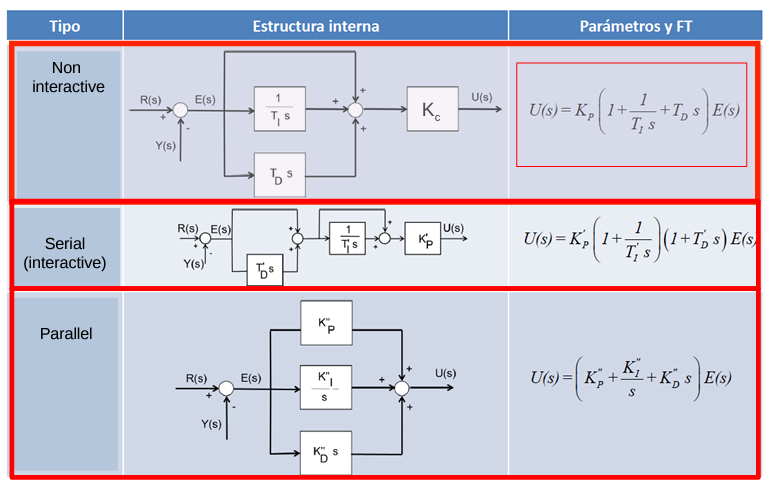
\includegraphics[width = 0.75 \textwidth]{Imagenes/3 - PID Types.png}
\end{figure}

\subsection{Proportional control: P}
Proportional control $K_p$ makes the response speed faster, which is desirable, but it increases the setling time.

A strong proportional control action increases the oscilation and inestability of the system. For safety reasons, overshooting should not exceed 30\%.

The proportional part does not consider time, therefore, the best way to solve the permanent error and consider the variation with respect to time, is to include and set the integral and derivative actions.

\subsection{PD Controller}
PD control with $K_p$ and $T_d$ gains reduces the response speed and the setling time. 

The $T_d$ parameter increases the stability of the system, reducing the oscillations caused by the proportional component $K_p$.

The derivative action manifests itself when there is a change in the absolute value of the error. 

The function of the derivative action is to correct the error proportionally with the same speed as it is produced, this way it prevents the error from increasing.

\subsection{PI Controller}
PI control with $K_p$ and $T_i$ gains increases the response speed and setling time. 

The integral control mode is intended to decrease and eliminate the steady state error, caused by external disturbances and which cannot be corrected by proportional control.

The integral control acts when ther is a deviation between the variable and the set point, integrating this deviation in time and adding it ot the proportional action.

The integral control is used to avoid the inconvenience of an offset (permanent deviation of the variable with respect to the set point).

\subsection{PID Controller}
In general, when there is no knowledge of the process, the PID controller is the most controller. By properly is the most appropriate controller. By properly adjusting the three variables (gains) in the PID control algorithm, the controller can provide control actions tailored to the requirements of the specific process.

The response of the controller can be described in terms of control response to an error, the degree to which the controller overshoots the set point, and the degree of system oscillation. Note that the use of PID control does not guarantee optimal system control or system stability.

PI controllers are particularly common, since the derivative actions is very sensitive to noise.

While PID controllers are applicable to most control problems, they can perform poorly in some particular applications. This is why specific adaptations and other advanced methods were proporsed.

Tuning a control loop meand adjusting the control system parameters to the optimum values for the desired control system response.

The optimal behavior to a process change or a setpoint change varies depending on the application.

The most effective method generally requires developing some form of the process model, then choosing P, I and D based on the dynamic model parameters. Manual tuning methods can be very inefficient. The choice of a method will depend on whether the loop can be ``switched off'' to adjust it, and on the response time of the system.

\section{Basic Control}
\subsection{1st PID design method: Pole-zero cancellation controller}

Transfer function of the processes without delay: 
\[\frac{K_p}{1 + t_p s}\]

For clarity purposes, we will denote the transfer function of the process (tank, boiler, heater, etc.) as $G_p(s)$.

The design of a controller for a transfer function of a process without delay follows the analytical design method of pole-zero cancellation.

The controller function for a first order system with no delay is of type PI (Proportional and Integral) and hence it has the following structure:
\[G_c(s) = K_c \left( 1 + \frac{1}{T_i s}\right) = \frac{K_c (T_i s + 1)}{T_i s}\]

Where:
\begin{itemize}
    \item $K_c$ is the proportional gain
    \item $T_i$ is the integral constant
\end{itemize}

\begin{figure}[H]
    \centering
    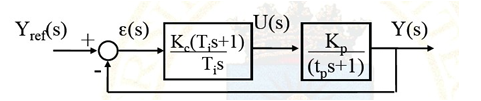
\includegraphics[width = 0.75 \textwidth]{Imagenes/3 - Pole-zero cancellation controller.png}
\end{figure}

The goal is to determine the controller parameters, $T_i$ and $K_c$.

\subsubsection{Design criterion.}
The design criterion is based on the closed-loop transfer function of the system, $M(s)$.
\begin{enumerate}
    \item If we set $T_i$ equal to the time constant of the process, $T_i = t_p$, then the closed loop controlled system behaves as a 1st order system:
    \[M(s) = \frac{Y(s)}{Y_{ref}(s)} = \frac{G_c G_p}{1 + G_c G_p} = \frac{K_c K_p}{t_p + s + K_c K_p} = \frac{1}{1 + \frac{t_p}{K_c K_p}s} = \frac{1}{1 + t_c s}\]
    \item The closed-loop time constant, $t_c$ is chosen by the designer.
    \item The controller gain is obtained from the closed-loop equation $M(s)$
    \[t_c = \frac{t_p}{K_c K_p} \rightarrow K_c = \frac{t_p}{K_p t_c}\]
\end{enumerate}

\subsection{2nd Controller Design Method: Processes with a delay}
Transfer function of the processes with delay:
\[\frac{K_p}{1 + t_p s} e^{-t_m s}\]

For clarity purposes, we will denote the transfer function of the process (tank, boiler, heater, etc.) as $G_p(s)$.

The design of controllers for processes with a deadtime is empirical and its based on tables, for example the Ziegler-Nichols (Z-N) tables or the AMIGO tables.

\subsubsection{Open-loop Z-N table (rules) based method}

The open-loop Z-N rules, published in 1942, were obtained by experimenting with a large number of simulated system on an analog simulator from the Taylor Instrument company, and on the Differential Analyzer, an MIT's analog computer.

The authors studied P, PI and PID controllers. To understand the process the followed, we will focus on the PI controller. For each of the simulated systems, the authors obtained two sets of data:
\begin{itemize}
    \item Descriptive data on the dynamic behavior of the simulated process ($G_p(s)$ parameters)
    \item PI regulator parameters ($K_c$ and $T_i$), obtained by trial and error, which gave optimum loop performance.
\end{itemize}

1/4 error signal decay rate in response to a step in the distrubance variable.

They then correlated the data from the first group with those from the second group for the different systems simulated, to obtain laws or rules that would make it possible to determine, from the data describing the dynamic behavior of a process, the parameters of the PI controller that gave optimum operation of the loop. The same was done for P and PID type controllers.

This was done for two different ways of describing the dynamic behavior of a simulated process: the step response of the open chain process and the response of the closed loop with a P regulator and a controller gain that makes the loop critically unstable.

\begin{enumerate}
    \item Firstly, an FOPDT Model must be obtained by applying the previously presented methods.
    \[G_p (s) = \frac{K_p}{1 + t_p s} e^{-T_t s}\]
    \item The followin parameters are extracted from the FOPDT model of the system to be controlled:
    \begin{itemize}
        \item $K_p$: Static gain
        \item $T_t$: Delay Time
        \item $T_p$: Time constant
    \end{itemize}
    \item With the $K_p$, $T_p$ and $T_t$ parameters, go to the Z-N table and calculate the parameters for the controller type of your choice: P, PI or PID.
\end{enumerate}

\begin{figure}[H]
    \centering
    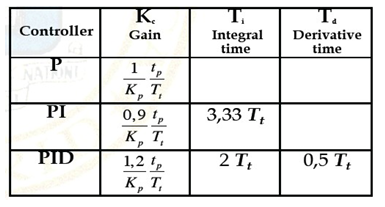
\includegraphics[width = 0.5 \textwidth]{Imagenes/3 - Open Loop Z-N table.png}
\end{figure}

The operation range for Z-N Open Loop tables:
\[ 0.1 \leq r = \frac{T_t}{t_p} \leq 0.9 \]

\subsubsection{Two methods to obtain the FOPDT function}
\begin{enumerate}
    \item FOPDT obtained by linearization of the system equations (Analytical function method) + multiplication by the existing delays. This only applies if the system + actuator system if a 1st order system.
    \item FOPDT obtained by the graphical method of the tangent and 63\%, based on an experimental curve resulting from a 10\% increment in the considered input signal.
\end{enumerate}

\subsubsection{The MIGO method}
MIGO stands for ``M-constrained Integral Gain Optimization''. This method comes from the Åström group (Lundt University, Sweden) and was published in the last years of the 20th century.

In this method, the PID controller parameters are calculated so that the integral gain of the PID controller is maximized, while keeping the robustness of the controller within given levels.

Maximize $K_c/T_i$ while keeping the relative stability above a threshold, in response to a step in the distrubance variable.

\subsubsection{The AMIGO method}
Optimization of the MIGO method is performed by individually for each process, based on its tf, which is laborious in a plant where there may be hundreds of control loops. To facilitate the tuning of conttollers, the AMIGO rules were developed from the MIGO method.

AMIGO is the acronym for Approximate MIGO. It is a set of rules for PI and PID controllers, dating from 2002 and 2004; they are dur to Åström and Hägglund.

These rules follow the philosophy of the Ziegler-Nichols rules. First a large set of tfs, representative of those appearing in process control (9 different types of tfs, which when parametrerized give a total of 134 tfs), was developed.

For each of the aforementioned tfs, the authors obtained:
\begin{itemize}
    \item descriptive data on the dynamic behavior of the tfs.
    \item parameters of the optimum regulator according to the MIGO method
\end{itemize}

They the correlated the data of the first group with those of the second group for the different systems simulated, in order to try to obtain laws or rules that would make it possible to determine from the descriptive data of the dynamic behavior of a process, the parameters of the regulator that gave an optimal operation of the loop.

\begin{figure}[H]
    \centering
    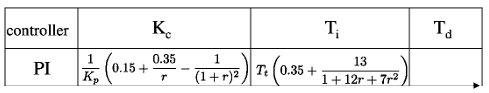
\includegraphics[width = 0.5 \textwidth]{Imagenes/3 - AMIGO rules for PI Controller.png}
\end{figure}

\[r = \frac{T_t}{t_p}\]

Where $K_p$, $T_t$, and $t_p$ are the parameters of the FOPDT model of the process, generally obtained by the tangent and the 63\% method.

The approximation between the results obtained with the MIGO method and those obtained with these AMIGO rules is very good.

\begin{figure}[H]
    \centering
    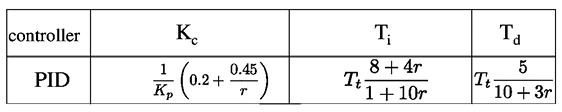
\includegraphics[width = 0.5 \textwidth]{Imagenes/3 - AMIGO rules for PID Controller.png}
\end{figure}

The approximation between the results obtained with the MIGO method and those obtained with the AMIGO rules for $K_c$ and $T_i$ is very good for $r \geq 0.25$ and conservative for $r < 0.25$. ``Conservative'' means that the error separates us from the optimal solution given by MIGO but still keeping the loop within the recommended values of robustness.

The approximation for $T_d$ is very good for $r \geq 1$ and conservative for $r < 1$.

Operation range for AMIGO tables: 
\[0.25 \leq r = \frac{T_t}{t_p} < 3\]

\subsubsection{The closed-loop ZN method}
The fourth method of controller design is based on the closed-loop ZN rules.

In this case the controller design strategy is to close the loop of a process using a proportional controller with gain $K_c$, as illustrated in the figure below.

\begin{figure}[H]
    \centering
    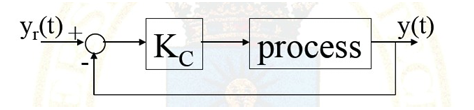
\includegraphics[width = 0.5 \textwidth]{Imagenes/3 - Closed Loop ZN.png}
\end{figure}

The design method consists of the following steps:
\begin{enumerate}
    \item Vary the gain $K_c$ of the closed-loop system until the output oscilates in a sustained manner, as shown in the attached figure. We will denote this gain value the ultimate gain $K_u = K_c$.
    \item Based on the oscillatory output curve we measure on the curve the perior $T_u$, which we will call, the ultimate period.
    \item Determine the parameters of the PID controller from the table.
\end{enumerate}

\section{Controller design improvements}
\subsection{Anti-windup filter}
As a result of the actuators saturation, the steady state error remains and the integral control output may accumulate very high values. In our tank systems, the elements that may present a saturation are the valves.

The adverse effect of the integral component generally occurs when the error is very high and is maintained for a long time. In this case the system is saturated and the integral control cannot perform its function.

In these cases it is recommended to disable or attenuate the intergal control by means of a filter so that excessive overshoot does not occur.

There are serveral way to implement the anti wind-up control, here we will study the one illustrated in the figures below.

\begin{figure}[H]
    \centering
    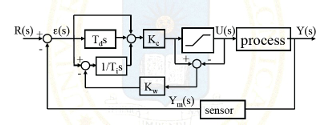
\includegraphics[width = 0.5 \textwidth]{Imagenes/3 - Anti-windup filter.png}
\end{figure}